\chapter{Methodology and Experimental Framework} \label{ch:methodology}
\section{Experimental framework}
Q1 attributes a plot's deviation from the baseline growth curve to environmental and management factors. Q2 tests whether spatially varying relationships capture what global models miss. Finally, Q3 evaluates whether these signals improve top-height predictions.

\begin{table}[!ht]
\centering
\footnotesize
\renewcommand{\arraystretch}{1.15}
\begin{tabularx}{\linewidth}{@{} l >{\raggedright\arraybackslash}X >{\raggedright\arraybackslash}X >{\raggedright\arraybackslash}X @{}}
\toprule
Q & Unit and target & Models or comparison & Main evaluation \\
\midrule
Q1 & Plot; mean pooled-CR residual & Elastic Net, XGBoost and two-stage
mixed-effects model & Five-fold spatial block CV; coefficients, SHAP and residual Moran's $I$ \\
Q2 & Plot; difference between fitted and yield-class-implied asymptotes & Elastic Net, XGBoost
and GNNWR & Five-fold spatial block CV; attribution, Moran's $I$ and target audit \\
Q3 & Plot--survey row; 95th-percentile top height, and row-level error reduction against the
fold-matched CR curve & CR, linear regression, random forest, XGBoost, DNN, PINN and PINN-$k$
& Five-fold spatial block CV; random-split and PINN forward-pass diagnostics; CR-error-quartile
correction with permutation control \\
\bottomrule
\end{tabularx}
\caption{\small{Units, targets and evaluation used for each question. Q3's row-level CR-error-quartile
check reuses Q3's own model predictions (conditioned DNN, PINN, PINN-$k$ and XGBoost) rather
than introducing a separate comparison.}}
\label{tab:rq-framework}
\end{table}

\paragraph*{Data partitions and leakage control}
The four-survey cohort served as the main dataset, while the six-survey cohort was kept as a longer-term sensitivity check. For Q1 and Q2, each plot had one summary value, while Q3 used every plot-survey row.

Spatial-block cross-validation prevented data leakage by assigning whole forest compartments to folds, ensuring no compartment appeared in both training and testing \cite{roberts2017Cross_C5_EVAL}. Training plots within 60\,m of validation or test plots were also removed to prevent spatial spillover. Five folds of roughly equal size were created. In each round, three folds trained the model, one fold tuned it, and one fold tested it. Each compartment was tested exactly once, and all test predictions were combined to calculate final performance metrics \cite{ploton2020Spatial_C5_EVAL}.


\begin{figure}[!htbp]
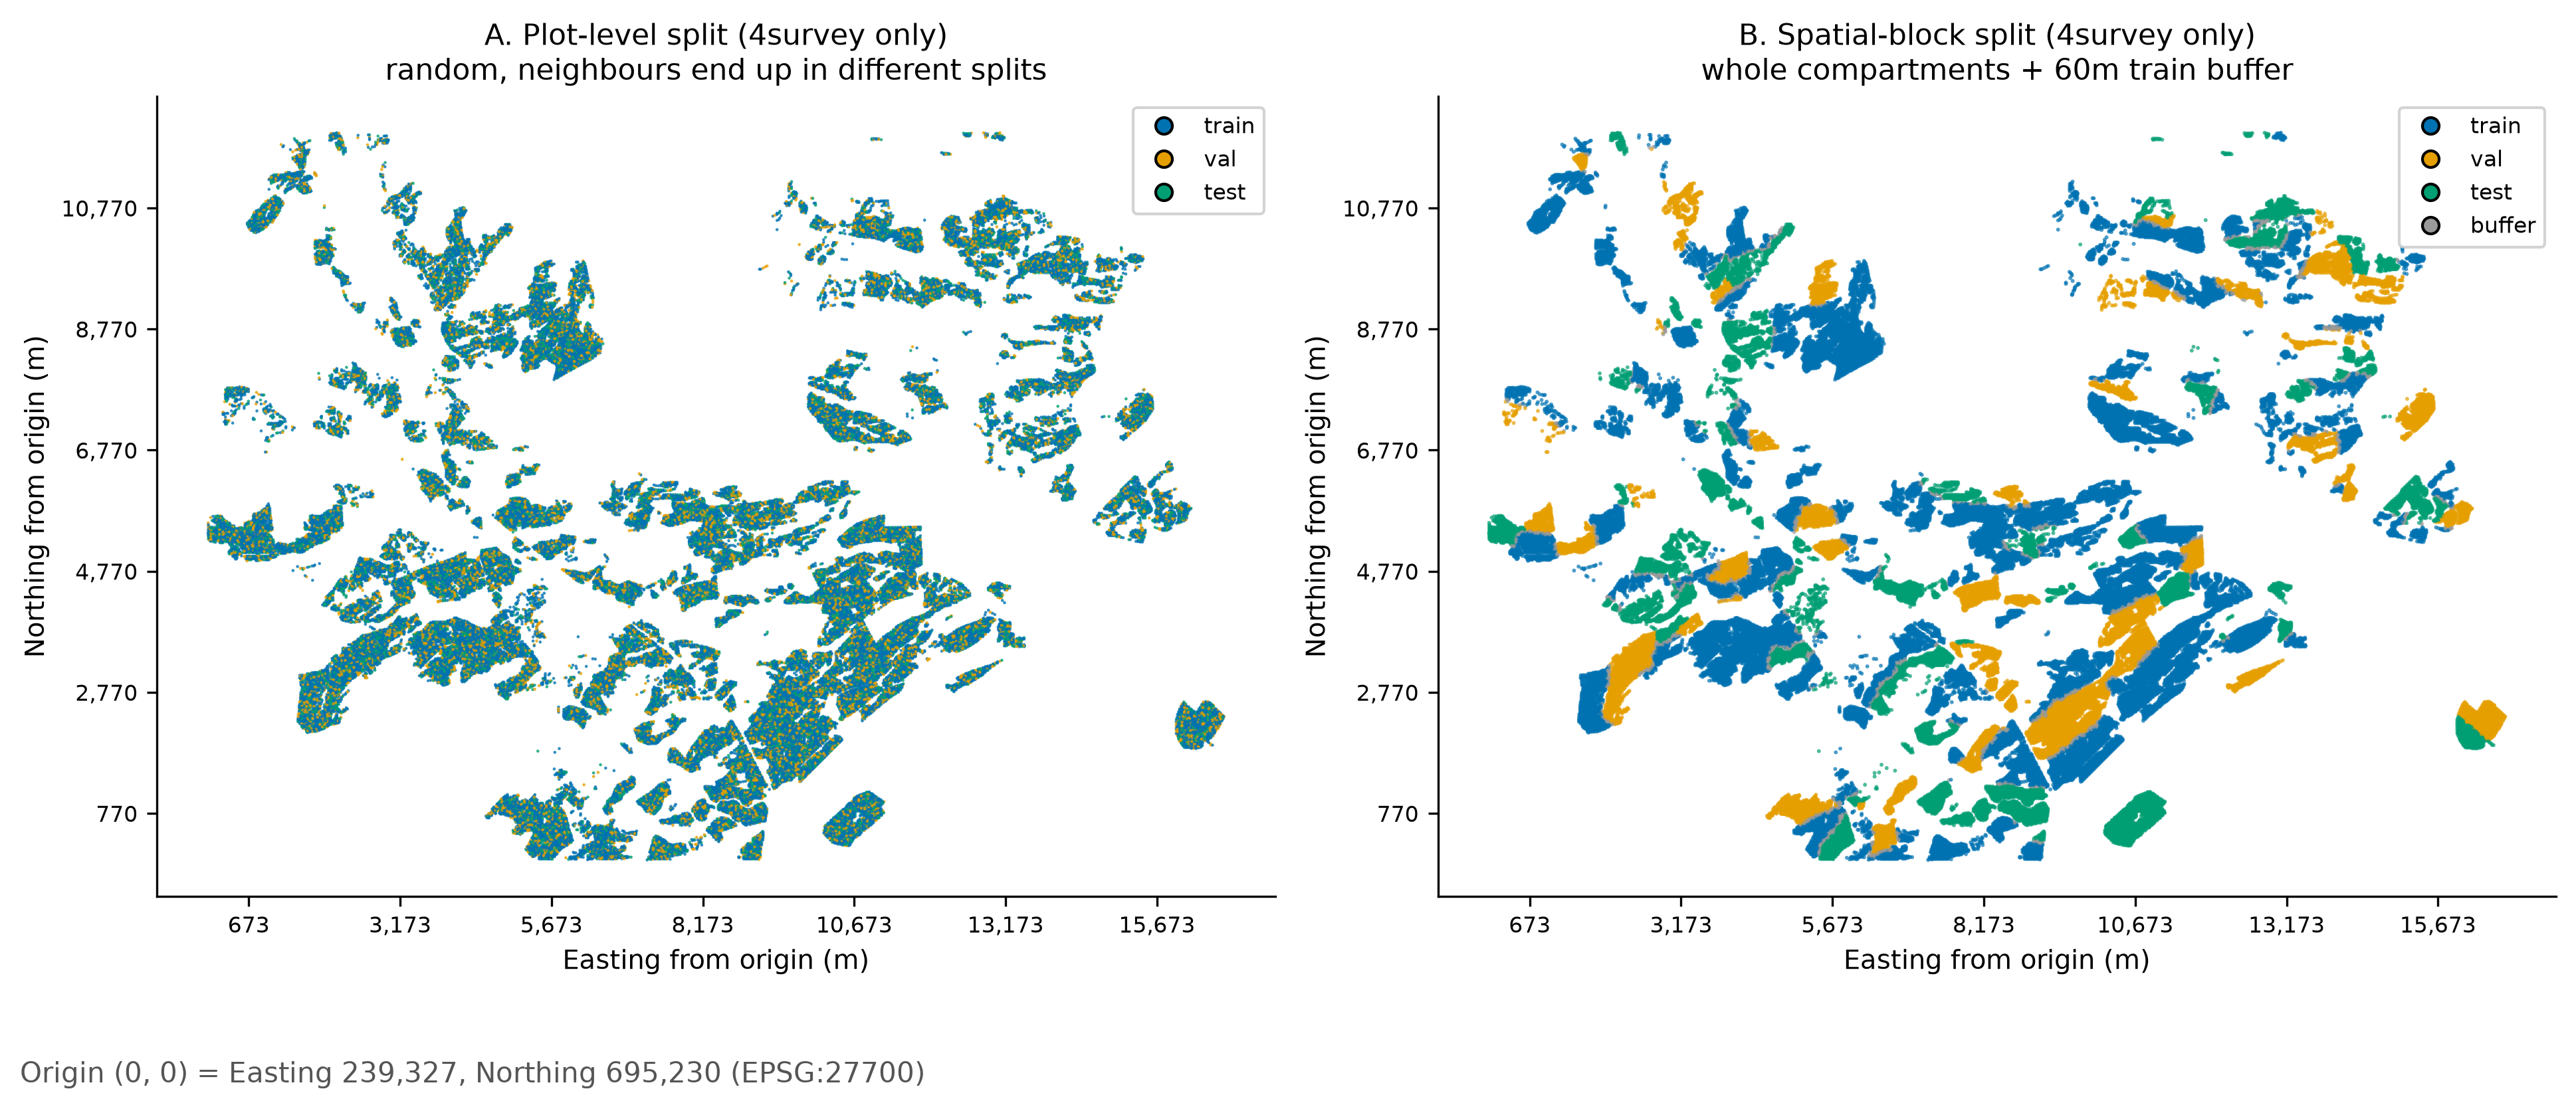
\includegraphics[width=1.0\textwidth]{figures/fig_methodology/fig_method_map_splits.png}
\centering
\caption{\small{Evaluation data-splitting strategies: (A) random plot-level split and (B) compartment-level spatial-block split with a 60\,m buffer.}}
\label{fig:splits-combined}
\end{figure} %TODO: increae font size. for axis. 

Continuous variables were scaled using the training data and applied to the validation and test sets. Age was scaled on its own so PINN outputs could be turned into metres per year. Soil types were converted into binary categories. Compartment and block IDs were left out of the models. Two neighbour-height variables were also dropped because they were made using nearby plot heights before the split, which could leak test answers.

\section{Q1: Explaining growth deviations}
Q1 uses the four-survey cohort because the six-survey cohort has too few compartments for spatial testing. Here, $i$ marks a plot, $t$ marks a survey, $H_{it}$ and $a_{it}$ are observed height and age, and $T_i$ is the number of surveys for plot $i$.  $H(a)$ is the shared Chapman-Richards growth curve (Equation~\eqref{eq:cr}) at age $a$. Equation~\eqref{eq:cr-gap} computes the gap between measured height and the baseline curve, while Equation~\eqref{eq:mean-cr-residual} averages this gap over time to give one persistent growth departure per plot:
\begin{align}
r_{it} &= H_{it} - H(a_{it}), \label{eq:cr-gap} &
\bar{r}_i &= \frac{1}{T_i} \sum_{t=1}^{T_i} r_{it}. \label{eq:mean-cr-residual}
\end{align}
A positive $\bar{r}_i$ indicates a plot that consistently outgrows the regional baseline. Stand age is omitted from model predictors since the growth curve already accounts for it.

We test Elastic Net and XGBoost using five-fold spatial cross-validation. Elastic Net tunes its penalty parameters on each training fold using an inner loop. XGBoost uses tuned parameters (depth 4, learning rate 0.04, up to 500 trees with early stopping). Performance is measured using pooled out-of-fold $R^2$.

To account for plots grouped within compartments, we fit a two-stage mixed-effects model. Stage~1 extracts $\bar{r}_i$ from the baseline curve. Stage~2 fits:
\begin{equation}
\bar{r}_i = \boldsymbol{\beta}^{\top}\mathbf{x}_i + u_{c[i]} + \varepsilon_i,
\label{eq:mixed-effects}
\end{equation}
where $\boldsymbol{\beta}^{\top}\mathbf{x}_i$ represents fixed effects (landscape-wide relationships reported across all plots, such as slope or TOPEX), and $u_{c[i]} \sim \mathcal{N}(0, \sigma_u^2)$ is a random compartment intercept. The random intercept captures shared local conditions (such as microclimate or soil) by estimating the overall variance across compartments ($\sigma_u^2$), rather than fitting a separate parameter for each compartment.

Parameters ($\boldsymbol{\beta}$ and $\sigma_u^2$) are fitted using restricted maximum likelihood (REML), which avoids the slight variance underestimation seen in standard maximum likelihood (ML). However, when directly comparing models with different fixed effects to assess how much compartment variance the environmental predictors explain, ML is used instead, as REML likelihoods cannot be compared across different fixed-effect structures. Results are reported as mean $\pm$ standard deviation across folds.

Two concerns motivate four sensitivity checks; first, because canopy cover and top height come from the same LiDAR flights, a strong canopy-cover effect might reflect measurement overlap rather than true stand structure. We test this through three steps: (1) refitting Set~4 without canopy cover to assess the change in $R^2$; (2) checking direct correlations between canopy cover and each target; and (3) recalculating SHAP values without canopy cover to see if other predictors absorb its explanatory role. 

Second, differences in terrain coefficients (such as slope and TOPEX) between Elastic Net and mixed-effects models could reflect local, compartment-specific effects that global models miss. We test this with a fourth check: (4) measuring how much variance in slope and TOPEX occurs between compartments versus within them, identifying whether their spatial structure masks local relationships.

Comparing Elastic Net, mixed-model coefficients, and XGBoost SHAP values provides three complementary perspectives on growth drivers, while residual Moran's $I$ tests for remaining spatial clustering (Section~\ref{sec:eval-robustness}).


%------------------------------------------------
\section{Q2: Spatial attribution}
Because Q1 models left clustered errors across the landscape, we test whether allowing environmental relationships to vary across space improves explanatory power. We use GNNWR \cite{du2020Geographically_C6_GWR}, which uses a neural network to learn spatial weighting from geographic coordinates without fixing a rigid neighbourhood size.

However, GNNWR assumes local relationships are linear. If the true biological response is non-linear, fluctuating local coefficients may simply show that a straight line fits poorly in that area, rather than a real geographic difference in growth drivers. This does not impact the broader $R^2$ comparison, but individual local coefficients should be interpreted with caution.

\paragraph*{What Q2's target actually measures:} For each plot, does its own growth so far point toward a higher or lower height ceiling than its assigned yield class predicts? $p_1$--$p_5$ are Forest Research's own published numbers that convert a yield-class rating into a full growth curve for a species and region; this project did not derive them, only reused them. $p_4$ (growth rate) and $p_5$ (curve shape) are the same for every plot sharing a yield class, only the height ceiling is allowed to differ from plot to plot \cite{scolforo2013Dominant_C2_CR}. For plot $i$ at survey $t$:
\begin{align}
g_{it} &= \left(1-e^{-p_{4,i}a_{it}}\right)^{p_{5,i}}, \label{eq:git-curve} \\
\hat y_{\max,i} &= \frac{\sum_t H_{it}g_{it}}{\sum_t g_{it}^2}, \label{eq:plot-ymax-fit} \\
y_{\max,i}^{\mathrm{yldc}} &= \mathrm{yldc}_i p_{2,i}+p_{1,i}+2p_{3,i}, \label{eq:yldc-asymptote} \\
\Delta y_{\max,i} &= \hat y_{\max,i}-y_{\max,i}^{\mathrm{yldc}}. \label{eq:local-ymax-diff}
\end{align}
Equation~\eqref{eq:plot-ymax-fit} fits each plot's own height ceiling, $\hat y_{\max,i}$, from that plot's own measured heights over time (using a fitting method, ordinary least squares through the origin, chosen because it stays stable even with only 4--6 survey measurements, and letting the rate and shape vary per plot too would need more data than most plots have). Equation~\eqref{eq:yldc-asymptote} works out the ceiling the plot's assigned yield class would predict, $y_{\max,i}^{\mathrm{yldc}}$, using that same fixed rate and shape. The target, $\Delta y_{\max,i}$ (Equation~\eqref{eq:local-ymax-diff}), is simply the difference between the two.

The value $\Delta y_{\max,i}$ summarises each plot across survey years. Positive values show growth toward a higher height ceiling than expected by yield class, and negative values show a lower ceiling. Here, $\hat{y}_{\max,i}$ is an estimated ceiling rather than an observed height. All plots within a cohort share the exact same measurement period (15 years for 4 surveys; 21 years for 6 surveys). With curve rate and shape parameters held constant, all local growth differences are captured in $\hat{y}_{\max,i}$. 

Following the Q1 setup, Elastic Net and XGBoost are trained on $\Delta y_{\max}$ using Sets~2--4. Spatial variation is modelled using GNNWR via its Python library \cite{du2020Geographically_C6_GWR, du2022PyGNNWR_C6_GWR}:
\begin{equation}
\hat{y}_i = \beta_0(s_i) + \sum_j \beta_j(s_i) x_{ij}.
\label{eq:gnnwr}
\end{equation}
GNNWR begins with a baseline linear model and learns how feature effects vary across space. For location $s_i$, a neural network converts distances to training plots into local coefficient adjustments without pre-set search radii. All main models use the full training data across the five spatial folds.

\subsection*{Computational adjustments and feature evaluation}
Two separate GPU limits affected GNNWR. First, calculating distances to all $\sim$31,000 training plots ran out of memory on a 10.57\,GiB GPU. Early tests used a smaller reference set sampled across compartments, but moving to a larger GPU allowed full, uncapped runs for all main results. Subsampling was kept only to test whether data sparsity drove six-survey instability. Second, GNNWR's built-in tool builds a hat matrix for AIC and $F$-tests, which exceeded memory on large runs. Disabling this step avoided crashes without altering reported $R^2$ or RMSE; AIC values use raw feature counts and $F$-tests are omitted. Elastic Net and XGBoost were unaffected.

Feature importance is assessed via XGBoost gain and test-fold SHAP values \cite{lundberg2017unified}. % Lundberg & Lee (2017) for SHAP
Predictors are also grouped into terrain, wind, soil, climate, and location sets to test their impact on $R^2$ and residual Moran's $I$ (Set~4, 4-survey cohort).

\subsection*{Target and outlier audit}
To remove bad data, plots are dropped if consecutive surveys match either rule:(1) Clearfell: Top height drops $\ge 25\%$, canopy cover drops $\ge 70\%$, and standing volume drops $\ge 70\%$.
(2) Measurement error: Top height drops $\ge 25\%$, while canopy cover drops $\le 10\%$ and volume does not drop. Plots with large height drops that match neither rule are kept. Extreme fitted ceilings ($\hat{y}_{\max,i}$) are identified using Tukey's $1.5\,\mathrm{IQR}$ rule \cite{tukey1977exploratory}: % Tukey (1977)
\begin{equation}
\left[Q_1 - 1.5\,\mathrm{IQR},\; Q_3 + 1.5\,\mathrm{IQR}\right].
\label{eq:tukey-fences}
\end{equation}
Fences are set separately per cohort following standard forest growth modelling practices \cite{weiskittel2011forest}. % Weiskittel et al. (2011)
Flagged plots are retained in primary runs, but evaluated in a sensitivity test by removing them from test predictions.

The audit checks if the top 1\% and 5\% largest residual plots overlap across Elastic Net, XGBoost, and GNNWR. We test their spatial distribution, distance to stand edges, wind shelter, and local coefficients against standard plots, and refit them without 2008 data to see whether errors stem from fitting artifacts or true ecological trends.

%------------------------------------------------
\section{Q3: Prediction and physics guidance}

Q3 tests if environmental variables improve top-height predictions and evaluates physics-informed neural networks. Using five spatial folds on Set~3, we compare a baseline growth curve, standard tabular models, and neural networks, using the other feature sets to test the benefit of adding environmental data.

\subsection{Chapman--Richards (CR) baseline}
\begin{equation}
H(a) = y_{\max}\left(1 - e^{-ka}\right)^p,
\label{eq:cr}
\end{equation}
where $H(a)$ is height at age $a$, $y_{\max}$ is the height asymptote, $k$ is the growth rate, and $p$ controls curve shape. All three parameters are fit freely by non-linear least squares on each training fold and frozen, keeping test folds fully independent.

\subsection*{Conventional models}
We test three baselines: linear regression, random forest, and XGBoost [1]. For Q3, XGBoost was tuned across 27 parameter settings over five folds using validation $R^2$ (Appendix~\ref{app:hyperparameters}).

\subsection{DNN and physics-informed models}
All neural networks use a three-layer trunk (128 units per layer, Leaky-ReLU) trained with Adam (learning rate $10^{-4}$, weight decay $10^{-5}$, batch size 256, early stopping). The standard DNN minimizes mean squared error ($\mathcal{L}_{\mathrm{data}} = \frac{1}{N}\sum (\hat H_i-H_i)^2$). In the conditioned DNN, environmental variables feed directly into the input. In PINN models, they feed into auxiliary networks that guide the loss functions instead of the prediction trunk.

Equations~\eqref{eq:cr-derivative}--\eqref{eq:total-loss} define the physics-informed loss framework:
\begin{align}
H'(a) &= y_{\max}pk e^{-ka}\left(1-e^{-ka}\right)^{p-1}, \label{eq:cr-derivative} \\
\mathcal{L}_{\mathrm{phys}} &= \frac{1}{N}\sum_{i=1}^{N}\left(\frac{\partial\hat H_i}{\partial a_i}-H'(a_i)\right)^2, \label{eq:physics-loss} \\
\mathcal{L}_{\mathrm{traj}} &= \frac{1}{M}\sum_{j=1}^{M}\left(\frac{\hat H_{j,2}-\hat H_{j,1}}{\Delta a_j}-H'(\bar a_j)\right)^2, \label{eq:trajectory-loss} \\
\mathcal{L} &= \mathcal{L}_{\mathrm{data}} + \lambda_{\mathrm{phys}}\mathcal{L}_{\mathrm{phys}} + \lambda_{\mathrm{traj}}\mathcal{L}_{\mathrm{traj}} + 10^{-5}\sum_{\theta}|\theta|. \label{eq:total-loss}
\end{align}
Equation~\eqref{eq:cr-derivative} gives the theoretical growth rate. Equation~\eqref{eq:physics-loss} penalizes gaps between this rate and network derivatives ($\partial\hat H_i/\partial a_i$). Equation~\eqref{eq:trajectory-loss} penalizes differences across consecutive surveys from the same plot at midpoint age $\bar a_j$. The total loss in Equation~\eqref{eq:total-loss} balances these terms ($\lambda_{\mathrm{phys}}=\lambda_{\mathrm{traj}}=1$ by default; 0 disables physics). 

For conditioned PINNs, auxiliary networks adjust plot parameters:
\begin{equation}
y_{\max}^{(i)} = y_{\max}+f_y(\mathbf{x}_i), \quad k^{(i)} = k\exp\!\left(f_k(\mathbf{x}_i)\right).
\label{eq:param-adjust}
\end{equation}
\limit{In the evaluated implementation, $y_{\max}^{(i)}$ and $k^{(i)}$ guide the loss terms rather than passing directly into the prediction trunk; see Section~\ref{sec:rq1-pinn-limitation}.}

\subsection*{Row-level curve correction}
\label{sec:rq2a-method}
To test whether environmental inputs improve single plot--survey predictions, we measure absolute error reduction against the CR baseline:
\begin{equation}
d_i = \left|H_i-\hat H_i^{\mathrm{CR}}\right| - \left|H_i-\hat H_i^{\mathrm{model}}\right|.
\label{eq:residual-reduction}
\end{equation}
Positive $d_i$ indicates improvement. Test rows are split into baseline-error quartiles (Q1 best fit, Q4 worst fit) to see where gains concentrate. Two Set~3 XGBoost controls isolate this effect: removing environmental variables, and refitting from scratch on permuted environmental data. Spatial clustering of $d_i$ is checked with Moran's $I$.
%TODO: (do we do this and talk about it in q3, i dotn think so, if we dont lets drop it), or replace it witht he evaluations we do do? 


\section{Evaluation and robustness} \label{sec:eval-robustness}
Model accuracy is evaluated using RMSE, MAE, $R^2$, and Bias ($e_i = H_i - \hat H_i$):
\begin{equation}
\mathrm{RMSE}=\sqrt{\tfrac{1}{N}\textstyle\sum e_i^2}, \quad
\mathrm{MAE}=\tfrac{1}{N}\textstyle\sum |e_i|, \quad
R^2=1-\tfrac{\sum e_i^2}{\sum (H_i-\bar H)^2}, \quad
\mathrm{Bias}=\tfrac{1}{N}\textstyle\sum e_i.
\label{eq:eval-summary}
\end{equation}
Positive bias indicates under-prediction. We report fold-level means ($\pm\text{SD}$) or pooled metrics across all out-of-fold predictions. For the 4-survey cohort, $R^2$ $95\%$ confidence intervals are calculated using 1,000 compartment bootstrap resamples.

Residual spatial autocorrelation is measured using global Moran's $I$:
\begin{equation}
I=\frac{N}{W}\frac{\sum_i\sum_j w_{ij}(e_i-\bar e)(e_j-\bar e)}{\sum_i(e_i-\bar e)^2}.
\label{eq:morans-i}
\end{equation}
Spatial weights ($w_{ij}$) use binary, row-standardised distance bands matched to each model's semivariogram range (up to 5,000\,m; 999 permutations), subsampling 5,000 rows where necessary for computational efficiency. Moran's $I$ is omitted if semivariance is flat, and marked provisional if semivariance rises past 5,000\,m. Distances are reported alongside all values.